\documentclass{beamer}
\usepackage[russian]{babel}
\usetheme{metropolis}

\usepackage{amsthm, amssymb}
\setbeamertemplate{theorems}[numbered]

\setbeamercolor{block title}{use=structure,fg=white,bg=gray!75!black}
\setbeamercolor{block body}{use=structure,fg=black,bg=gray!20!white}

\usepackage[T2A]{fontenc}
\usepackage[utf8]{inputenc}

\usepackage{hyphenat}
\usepackage{amsmath}
\usepackage{graphicx}

\usepackage{booktabs}

\AtBeginEnvironment{proof}{\renewcommand{\qedsymbol}{}}{}{}

\title{
Микроэкономика-I
}
\author{
Павел Андреянов, PhD
}

\begin{document}

\maketitle

\begin{frame}{План на вторую часть лекции (1 час)}

Далее мы сфокусируемся только на полезностях и как оптимизировать их при различных ограничениях.

\begin{itemize}
  \item Начала оптимизации
  \item Условия первого и второго порядка
  \item Выпуклость задачи
  \item Краевые и внутренние решения
  \item Линии уровня и геом. анализ
\end{itemize}


\end{frame}

\section{Начала оптимизации}

\begin{frame}{Начала оптимизации}

Любая оптимизационная задача – это две вещи:

\begin{itemize}
  \item функция $U$ которую мы максимизируем
  \item область определения $X$ по которым мы максимизируем
\end{itemize}

Ключевыми факторами тут являются непрерывность и (квази-) вогнутость целевой функции, а также компактность и выпуклость области определения.

\end{frame}

\section{Существование}

\begin{frame}{Существование}

Существование решения, как правило, мы можем легко гарантировать при помощи следующей теоремы

\begin{theorem}[Вейерштрасса]

Непрерывная функция на (непустом) компакте гарантированно достигает своего минимума и максимума.
\end{theorem}

Что такое \alert{непрерывность} вы уже знаете, а \alert{компакт} в $\mathbb{R}^n$ - это просто ограниченное и замкнутое множество. 

В контексте одномерной оптимизации, отрезок $[a,b]$ - это компакт, а $(a,b]$, $[a,b)$, $(a,b)$, $[a,\infty)$,$(a,\infty)$ - нет. 

В экономике вам будут попадаться, в основном компакты, поэтому вопрос о существовании как правило стоит не остро.

\end{frame}

\section{Дифференциальный анализ}

\begin{frame}{Дифференциальный анализ}

Предположим, что функция на компакте не только непрерывна но еще и дифференциируема сколько угодно раз, такая задача называется \alert{гладкой}. Тогда оптимум может быть

\begin{itemize}
  \item либо на границе $X$
  \item либо во внутренней точке $X$
\end{itemize}

В последнем случае обязательно выполнены \alert{условия первого порядка} (УПП), это один из самых фундаментальных результатов дифференциального анализа.

\end{frame}

\begin{frame}{УПП}

Например, если функция $U(x, y, z)$ от трех переменных, и вы убедили себя, что решение надо искать внутри, то
$$\text{УПП (FOC)}: \quad  \nabla U = 0$$ 
должны выполняться в оптимальной точке $(x^{\ast}, y^{\ast}, z^{\ast})$. 

Значок $\nabla$ означает взятие градиента функции $$ \nabla U = \begin{pmatrix} \partial U/\partial x \\ \partial U/\partial y \\ \partial U/\partial z \end{pmatrix}$$
в соответствующей точке.

\end{frame}

\begin{frame}{УПП на границе}

Например, если функция $U(x, y, z)$, и вы убедили себя, что решение надо искать на границе $F(x,y,z) = 0$, то
$$\text{УПП (FOC)}: \quad  \nabla \mathcal{L} = 0, $$ 
где $\mathcal{L}(x,y,z|\lambda) = U(x, y, z) - \lambda F(x,y,z)$ это \alert{Лагранжиан}.

Значок $\nabla$ означает взятие градиента Лагранжиана по всем переменным включая множители Лагранжа $$ \nabla \mathcal{L} = \begin{pmatrix} \partial \mathcal{L}/\partial x \\ \partial \mathcal{L}/\partial y \\ \partial \mathcal{L}/\partial z \\ \partial \mathcal{L}/\partial \lambda \end{pmatrix}$$
в соответствующей точке.

\end{frame}


\begin{frame}{Критические точки}

Как правило, количество точек, в которых выполнены УПП, с Лагранжианом или без,  конечно. Оптимум может также находиться на каком-то изломе или иной аномалии границы области определения.

Все такие точки называются \alert{критическими}, их мало, и оптимум гарантированно лежит в одном из них. 

\end{frame}

\begin{frame}{Критические точки}

\begin{figure}[hbt]
\centering
\includegraphics[width=.8 \textwidth]{extrema.png}
\end{figure}

\end{frame}

\begin{frame}{Ручной перебор}

Если у вас по любой причине остался один кандидат, то он и является оптимумом, поскольку существование нам гарантирует Теорема Вейерштрасса. 

Если же кандидатов несколько, то надо сравнивать значения функции руками и выбирать все точки с наибольшим значением. 

Тупой перебор Критические точки может привести к неожиданно быстрому решению задачи.

\end{frame}

\begin{frame}{Пример 1}

Промаксимизируем функцию $f(x) = (x-1)^2$ на отрезке $[0,3]$.

\begin{itemize}
  \item Задача гладкая на компакте
  \item Решим УПП, получим первую критическую точку $x = 1$
  \item Две других критические точки это $x = 0$ и $x = 3$
  \item Сравним значения: $$f(0) = 1, \ f(1) = 0, \ f(3) = 4.$$
\end{itemize}

Получается, что в этой задаче один единственный оптимум в точке $x = 3$, причем до условий второго порядка у нас даже руки не дошли.

\end{frame}

\begin{frame}{УВП}

Число внутренних точек, прошедших УПП, можно дополнительно сузить за счет условий второго порядка.
$$\text{УВП (SOC)}: \quad  \nabla^2 U \ ? \ 0$$
Если Гессиан во внутренней точке отрицательно полу-определен $\nabla^2 U \leqslant 0$ (собственные значения $\leqslant 0$), то это \alert{локальный максимум} и этот кандидат проходит отбор.

Если Гессиан положительно определен $\nabla^2 U > 0$ (собственные значения $>0$), то это строгий \alert{локальный минимум} и этот кандидат точно не проходит отбор.

Есть еще третий случай, когда собственные значения Гессиана имеют противоположные знаки, это \alert{седло} и оно тоже не проходит отбор.

\end{frame}

\section{Выпуклость}

\begin{frame}{Выпуклость}

К счастью, в экономике зачастую удается показать, что поверх непрерывности функция полезности

\begin{itemize}
\item либо вогнутая
\item либо она монотонное преобразование вогнутой
\item либо она квазивогнутая
\end{itemize}

Если, вдобавок, область определения - выпуклое множество, то условия второго порядка можно не проверять. Такие задачи называются \alert{выпуклыми}.

\end{frame}

\begin{frame}{Пример 2}

Промаксимизируем функцию $f(x) = -(x-1)^2$ на отрезке $[0,3]$.

\begin{itemize}
  \item Задача гладкая и выпуклая на компакте
  \item Решим УПП, получим первую критическую точку $x = 1$
  \item Убедимся что он находится внутри области
\end{itemize}

Все, этот экстремум и есть решение.

\end{frame}

\begin{frame}{Пример 3}

Промаксимизируем функцию $f(x) = -(x+1)^2$ на отрезке $[0,3]$.

\begin{itemize}
  \item Задача гладкая и выпуклая на компакте
  \item Решим УПП, получим первую критическую точку $x = -1$
  \item Однако он не попадает в область, то есть, его нет
  \item Две других критических точки это $x = 0$ и $x = 3$
  \item Сравним значения: $$f(0) = 1, \ f(3) = -16.$$
\end{itemize}

Получается, что в этой задаче один единственный оптимум в точке $x = 0$.

\end{frame}

\begin{frame}{Выпуклость}

Очень важно уметь, глядя на задачу, определять выпуклая она или нет, чтобы не тратить время на анализ второго порядка. 

Общий алгоритм решения гладких и выпуклых задач на компакте очень простой:

\begin{itemize}
\item ищем первую критическую точку, как будто решение внутреннее
\item если не попало в область определения - ищем на границе
\item не забываем про изломы и иные аномалии области определения, потому что они, формально, являются кандидатами на решение
\end{itemize}

\alert{В выпуклых задачах условия второго порядка выполнены автоматически}, их проверка - пустая трата времени.

\end{frame}

\section{Геометрический анализ}

\begin{frame}{Линии уровня}

Наконец, линии уровня - это очень удобный инструмент для быстрого отлова и классификации кандидатов на решение оптимизационной задачи...

\begin{definition}
\alert{Линией уровня} полезности $U$, проходящей через точку $x$ называется множество всех точек $y \in X$ таких, что $U(y) = U(x)$.
\end{definition}

... особенно в двумерном случае.

\end{frame}

\begin{frame}{Кривые безразличия}

\begin{definition}
\alert{Кривой безразличия} предпочтений $\succcurlyeq$, проходящей через точку $x$ называется множество всех точек $y \in X$ таких, что $x \sim y$. Другими словами, это пересечение $L_+(x)$ и $L_-(x)$.
\end{definition}

Совершенно ясно, что в контексте представлений предпочтений полезностями, кривая безразличия и линия уровня - это одно и то же.

\end{frame}

\section{Локальная ненасыщаемость}

\begin{frame}{Локальная ненасыщаемость}

\begin{definition}
Предпочтения $\succcurlyeq$ \alert{локально ненасыщаемы} в $X$, если для любой точки $x \in X$ найдется сколь угодно близкая к ней точка $x' \in X$, такая что $x' \succ x$.
\end{definition}

\begin{definition}
Полезность $U$ \alert{локально ненасыщаема} в $X$, если для любой точки $x \in X$ найдется сколь угодно близкая к ней точка $x' \in X$, такая что $U(x') > U(x)$.
\end{definition}

Почти все полезности, которые будут вам встречаться, локально ненасыщаемы. Интуитивно это означает что кривые безразличия - тонкие линии. Если кривая безразличия толстая - это явное нарушение локальной ненасыщаемости.

\end{frame}

\section{Примеры полезностей}

\begin{frame}{Линейная полезность}

Рассмотрим полезность вида: $U(x, y) = ax + by$. Тогда линия уровня ищется следующим образом: 
\begin{gather*}
c = ax + by\\
c-ax = by\\
y = \frac{c-ax}{b}
\end{gather*}
Линия уровня - это прямая вида $y = \alpha x + \beta$.

Эта полезность гладкая, вогнутая и локально ненасыщаемая.

\end{frame}

\begin{frame}{Гиперболическая полезность}

Рассмотрим полезность вида: $U(x, y) = a \log x + \log y$. Тогда линия уровня ищется следующим образом: 
\begin{gather*}
c =  a \log x + \log y\\
e^{c} = x^a y\\
y =\frac{e^{c}}{x^a}
\end{gather*}
Линия уровня - это гипербола вида $y = x^\alpha \beta$.

Эта полезность гладкая, вогнутая и локально ненасыщаемая.

\end{frame}

\begin{frame}{Полезность минимум}

Рассмотрим полезность вида: $U(x, y) = \min(ax, by)$. Тогда линия уровня ищется следующим образом: 
\begin{gather*}
c = \min(ax, by)\\
\frac{c}{b}= \min(\frac{a}{b}x, y), \quad \frac{c}{a}= \min(x, \frac{b}{a}y)\\
y = \frac{c}{b} \mathbb{I}(ax > c), \quad x = \frac{c}{a} \mathbb{I}(by > c)
\end{gather*}
Линия уровня - это конкатенация горизонтальной и вертикальной линий, соединенных вдоль $ax = by$.

Эта полезность НЕгладкая, но непрерывная, вогнутая и локально ненасыщаемая.

\end{frame}

\section{Метод пристального взгляда}

\begin{frame}{Метод пристального взгляда}

Очень часто, в задачах есть выпуклое ограничение типа неравенства, например, бюджетное ограничение. A полезность вогнутая или квазивогнутая.

В таком случае, оптимум можно охарактеризовать как точку касания выпуклой области определения с одним из выпуклых верхних Лебеговых множеств. Однако, \alert{метод пристального взгляда работает только для локально ненасыщаемых предпочтений}. 

В маломерных задачах, эта точка ищется визуально, а точные ее координаты либо угадываются из симметрии, либо из каких то других соображений.

\end{frame}

\begin{frame}{Метод пристального взгляда}

\begin{figure}[hbt]
\centering
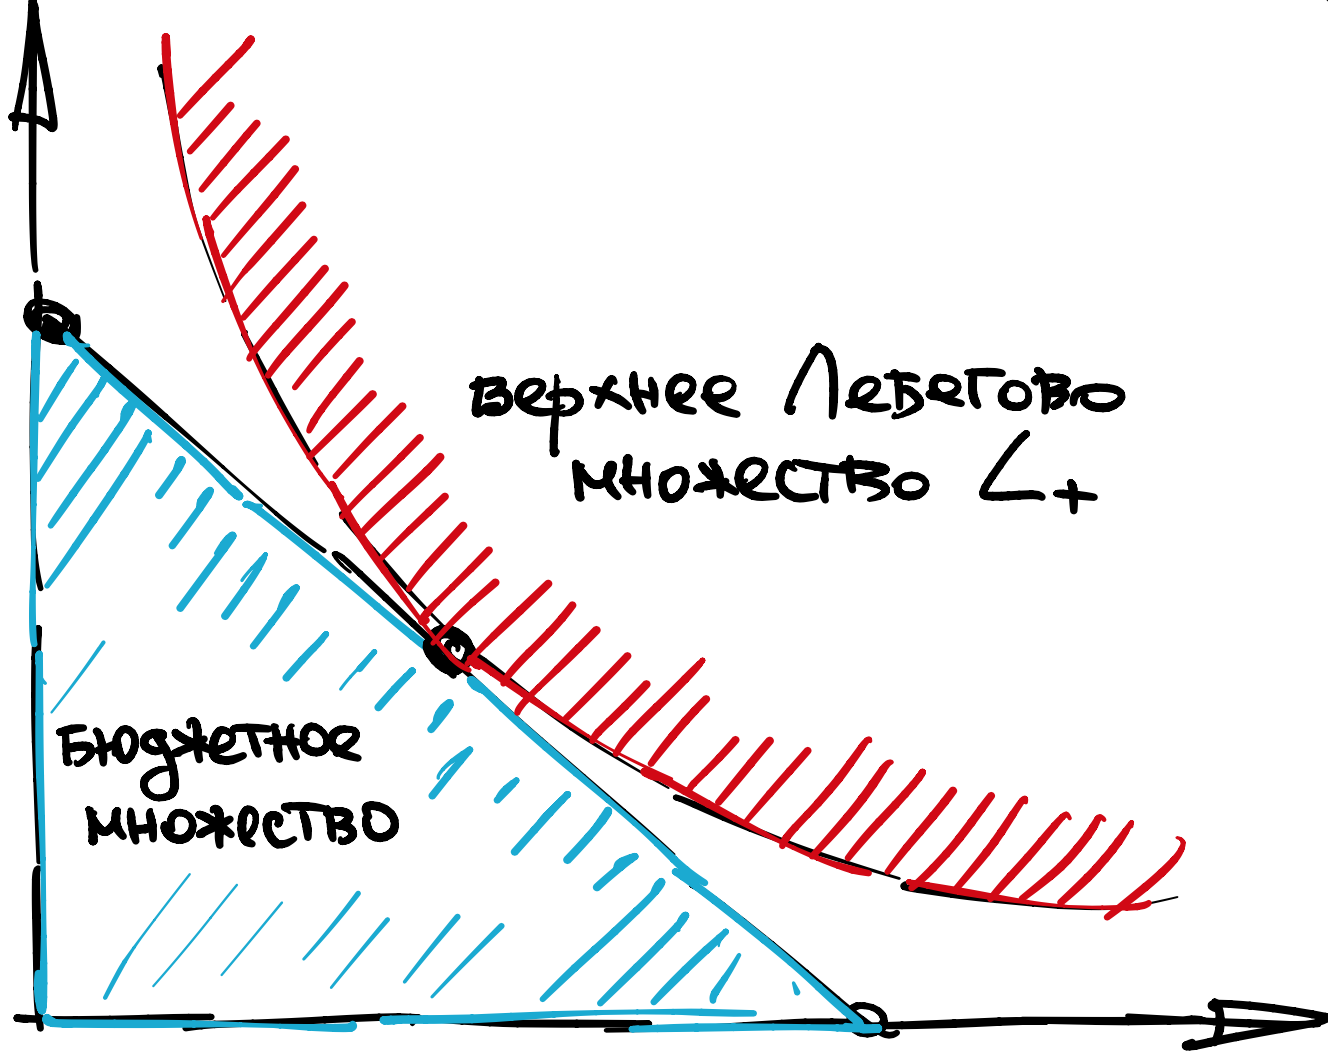
\includegraphics[width=.8 \textwidth]{tangency.png}
\end{figure}

\end{frame}
\begin{frame}{Метод пристального взгляда}

\begin{figure}[hbt]
\centering
\includegraphics[width=.8 \textwidth]{tang2.png}
\end{figure}

\end{frame}
\begin{frame}{Метод пристального взгляда}

\begin{figure}[hbt]
\centering
\includegraphics[width=.8 \textwidth]{tang3.png}
\end{figure}

\end{frame}

\section{Конец второй части лекции}

\end{document}